\documentclass{beamer}

\usetheme{PSU}
\usepackage{psu-colors}
\usepackage{psu-logos}

\usepackage{pgfplots, pgfplotstable}
\usepackage{amsmath, amssymb, amsthm, amsfonts}

\pgfplotsset{compat=newest}

\setmainfont{Acumin Pro}[
    UprightFont=*-Regular,
    BoldFont=*-Bold,
    ItalicFont=*-Italic,
]

\title{Organ voicing and flow-informed Ising number}
\subtitle{Team C -- CADES Lab}
\author[Cyanam, Nguyen, Pinochet-Soto]{Meghana Cyanam \and Hai Nguyen \and Gabriel Pinochet-Soto}
\institute{Portland State University}
\date{\today}

\begin{document}
    {
    \setbeamercolor{background canvas}{bg=psuForestGreen}
    \begin{frame}
		\titlepage
	\end{frame}
    }

    \begin{frame}
        \frametitle{Outline}
        \tableofcontents
    \end{frame}

    \section{Introduction}
    \subsection{What is organ tuning?}
	\begin{frame}
        \frametitle{Introduction: What is organ tuning?}
		\begin{itemize}
            \item
                Pipe organs have been around for hundreds of years, and making them sound just
                right is a special job called intonation, or \emph{voicing}.

			\item
                The way a pipe looks and is built -- like its size, shape, and material-- can
                change how it sounds.

			\item
                These details are decided first, and then the pipes are fine-tuned before being
                added to the organ.
		\end{itemize}
	\end{frame}

    \subsection{Good vs. bad voicing}
    \begin{frame}
        \frametitle{Introduction: Good vs. bad voicing}
        \begin{columns}
            \begin{column}{0.5\textwidth}
                \centering
                \begin{figure}[htbp]
                    \begin{tikzpicture}
                        \begin{axis}[
                            width=0.9\textwidth,
                            ybar,
                            xlabel={Partial},
                            ylabel={Relative amplitude},
                            symbolic x coords={1st, 2nd, 3rd, 4th, 5th, 6th, 7th, 8th},
                            ymin=0, ymax=100,
                            ytick={0, 50, 100},
                            tick label style={font=\large},
                            label style={font=\small},
                        ]
                          \addplot [
                            color=psuOrange,
                            fill=psuOrange,
                            opacity=0.75,
                        ] coordinates {(1st,99) (2nd,97) (3rd,97) (4th,81) (5th,64) (6th,45) (7th,30) (8th,12)};
                        \end{axis}
                    \end{tikzpicture}
                    \caption{\textbf{Good voicing}: Good distribution of harmonics.}
                    \label{fig:good_voicing}
                \end{figure}
            \end{column}
            \begin{column}{0.5\textwidth}
                \centering
                \begin{figure}
                    \begin{tikzpicture}
                        \begin{axis}[
                            width=0.9\textwidth,
                            ybar,
                            xlabel={Partial},
                            ylabel={Relative amplitude},
                            symbolic x coords={1st, 2nd, 3rd, 4th, 5th, 6th, 7th, 8th},
                            ymin=0, ymax=100,
                            ytick={0, 50, 100},
                            tick label style={font=\large},
                            label style={font=\small},
                        ]
                            \addplot [
                                color=psuOrange,
                                fill=psuOrange,
                                opacity=0.75,
                            ] coordinates {(1st,34) (2nd,99) (3rd,17) (4th,11) (5th,59) (6th,28) (7th,0) (8th,32)};
                        \end{axis}
                        \end{tikzpicture}
                    \caption{\textbf{Bad voicing}: Bad distribution of harmonics.}
                    \label{fig:bad_voicing}
                \end{figure}
            \end{column}
        \end{columns}
    \end{frame}

    \subsection{Ising number}
    \begin{frame}
        \frametitle{Introduction: Ising number}
        \begin{alertblock}{Ising number}
            \begin{equation}
                \label{eq:ising}
                \mathsf{I}
                =
                \frac{v}{\omega}\sqrt{\frac{d}{h^3}}
                =
                \frac{1}{\omega}\sqrt{\frac{2 P d}{\rho h^3}},
            \end{equation}
        \end{alertblock}
        \begin{enumerate}
            \item Can the Ising formula~\ref{eq:ising} be improved, refined, or
                corrected, in order to match measured data?
            \item Can the flow rate be included in the Ising formula~\ref{eq:ising}?
            \item Can we obtain a model reliable enough, that can be used to dimension the
                pipes before the voicing stage?
        \end{enumerate}
    \end{frame}

    \section{Action Plan}
    \subsection{Methodology}
    \begin{frame}
        \frametitle{Action Plan}
        \begin{enumerate}
            \item Semianalytical methods
            \item FEM simulations
            \item Machine learning (DNN) on JAX
            \item Generalized Additive Models (GAM)
        \end{enumerate}
    \end{frame}

    \section{Preliminary analysis}
    \begin{frame}
        \frametitle{Preliminary analysis: state of the data}
                \centering
                \begin{figure}[htbp]
                    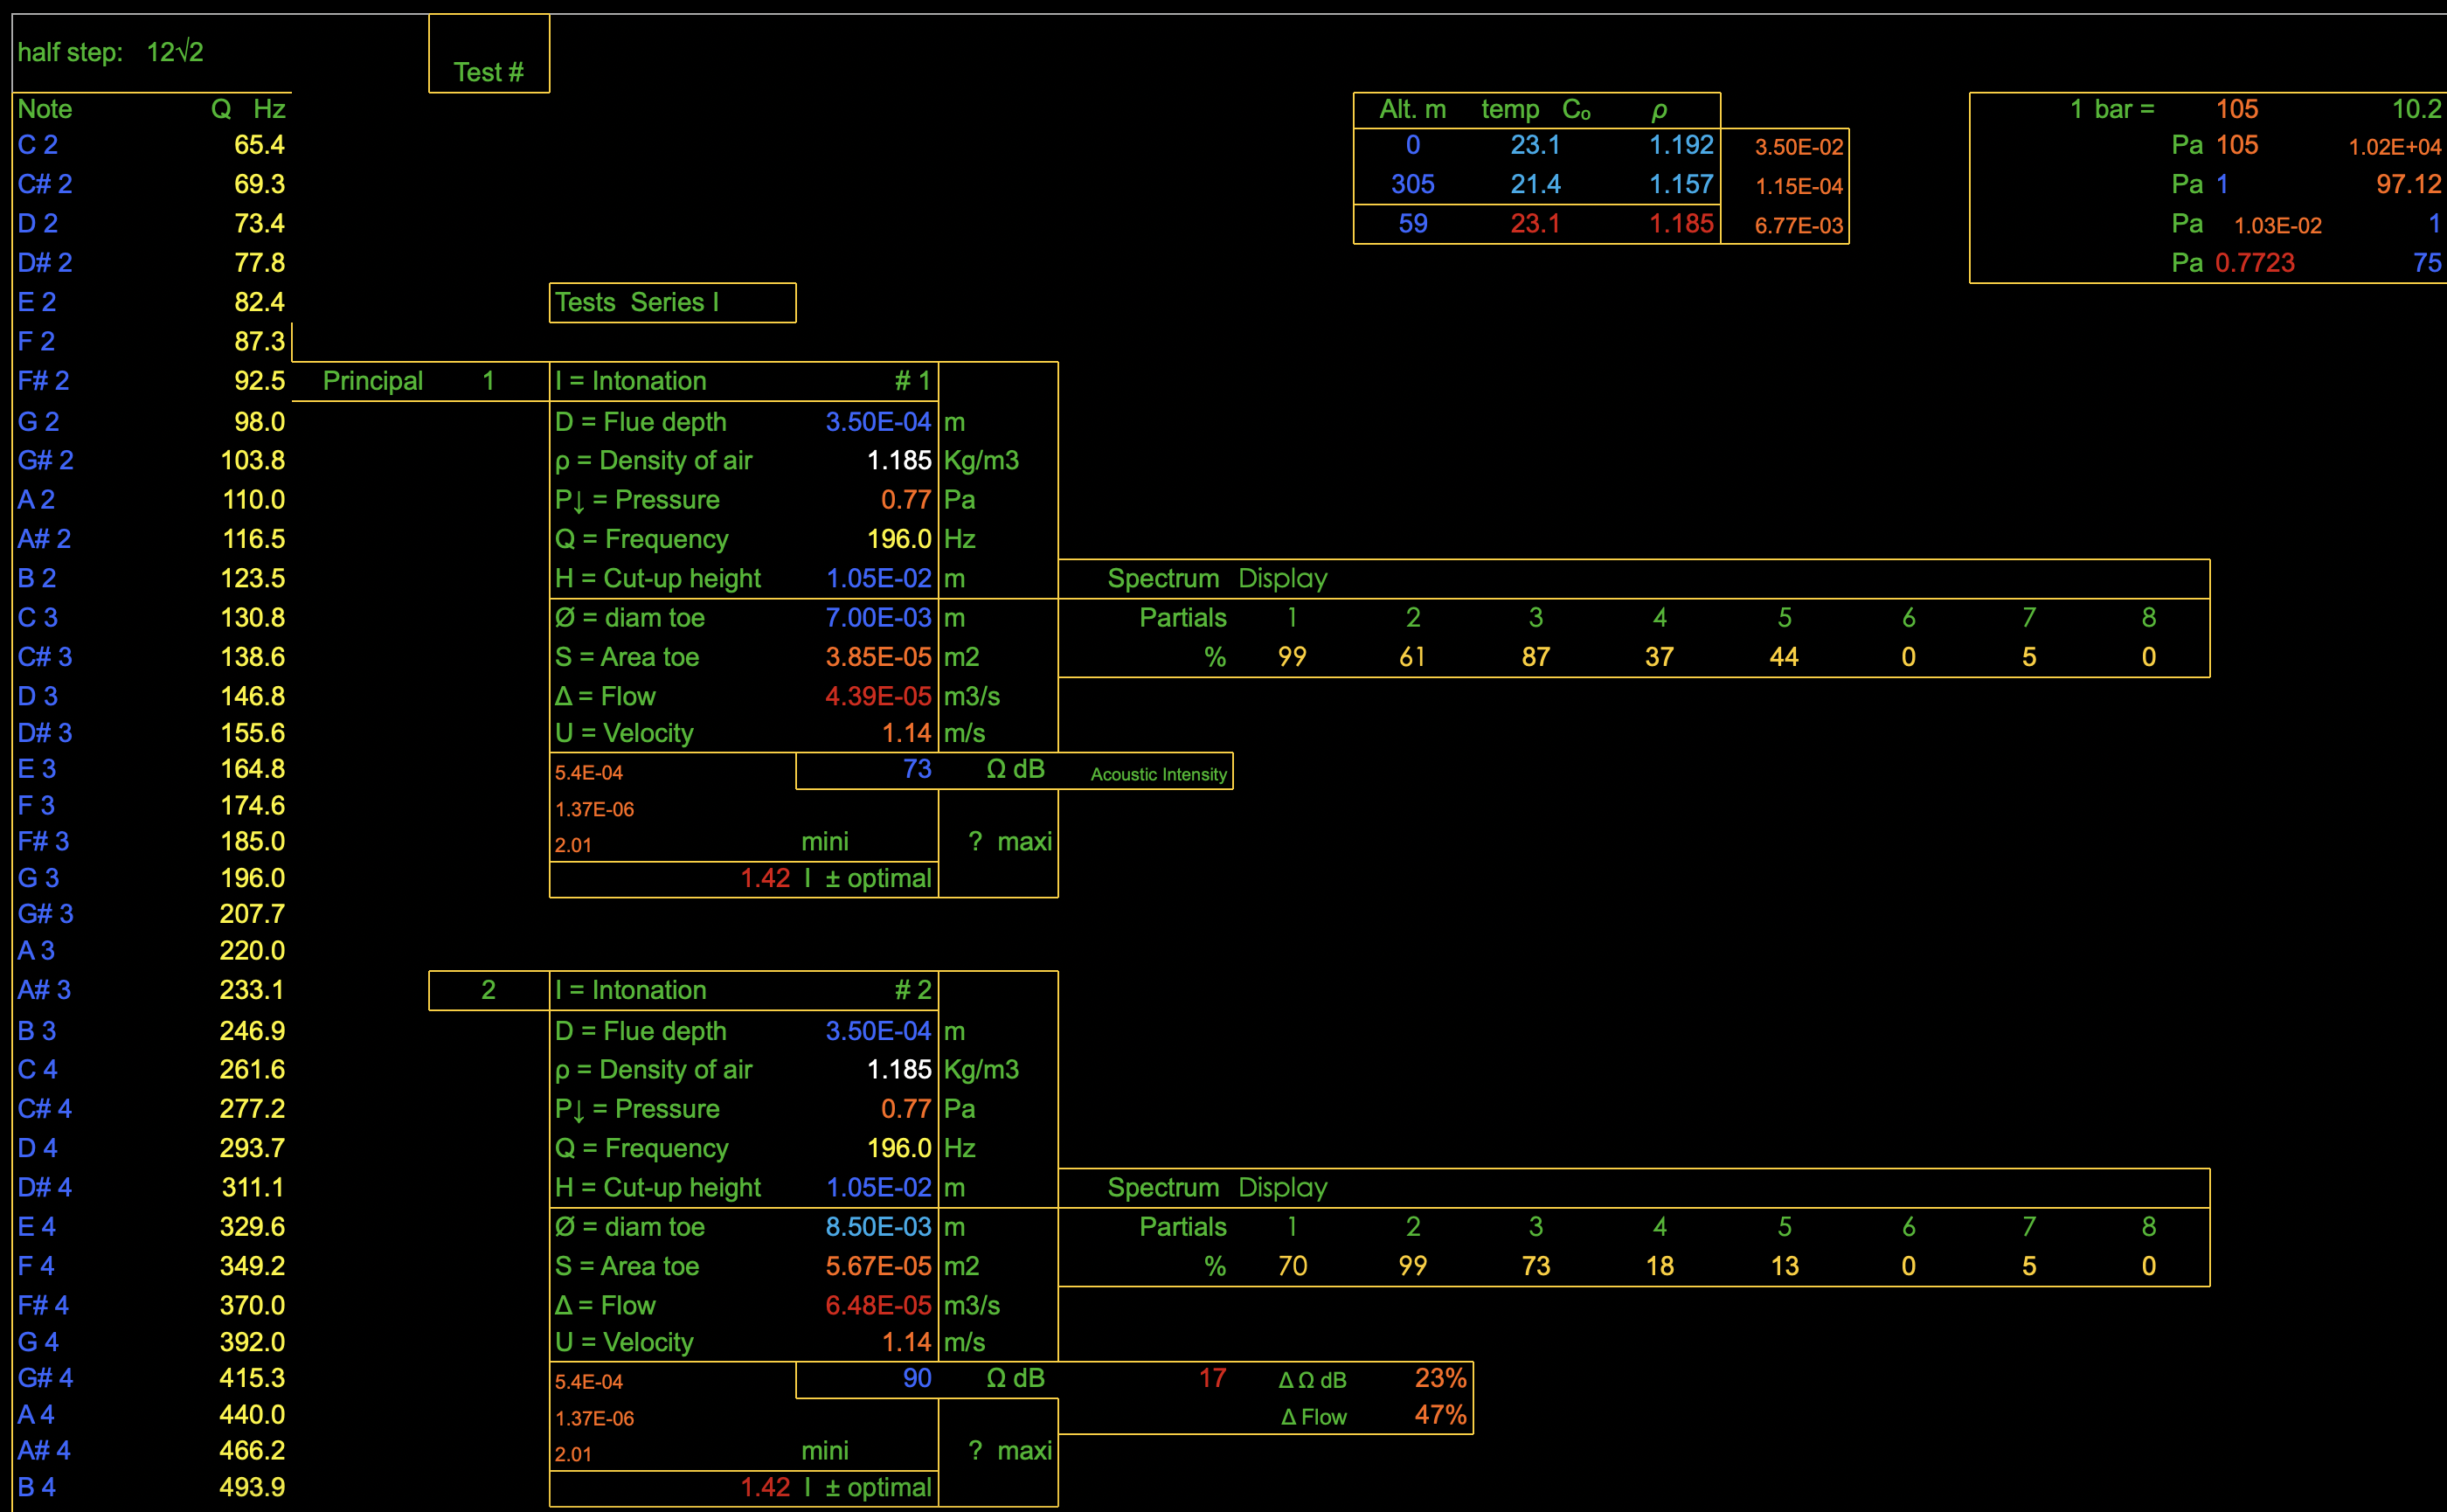
\includegraphics[width=0.9\textwidth]{pic1.png}
                    \caption{Initial state of the data}
                    \label{fig:initial_state}
                \end{figure}
    \end{frame}

    \begin{frame}
        \frametitle{Preliminary analysis: state of the data}
        \begin{columns}
            \begin{column}{0.5\textwidth}
                \begin{alertblock}{Initial state of the data}
                    \begin{itemize}
                        \item Redundant information \(\to\) remove constants,
                            known values.
                        \item Data is scarse \(\to\) small number of parameters.
                    \end{itemize}
                \end{alertblock}
                \begin{block}{Data}
                    \begin{itemize}
                        \item Convert to \texttt{.csv} format.
                        \item Pre-compute known values.
                        \item Define formulae for the Ising number.
                    \end{itemize}
                \end{block}
            \end{column}
            \begin{column}{0.5\textwidth}
                \begin{block}{Main objectives}
                    \begin{itemize}
                        \item Check the distribution of the partials.
                        \item Check for correlations.
                        \item Attempt simple corrections.
                        \item Attempt more complex modeling.
                    \end{itemize}
                \end{block}
            \end{column}
        \end{columns}
    \end{frame}

    \begin{frame}
        \centering
        \begin{figure}[htbp]
            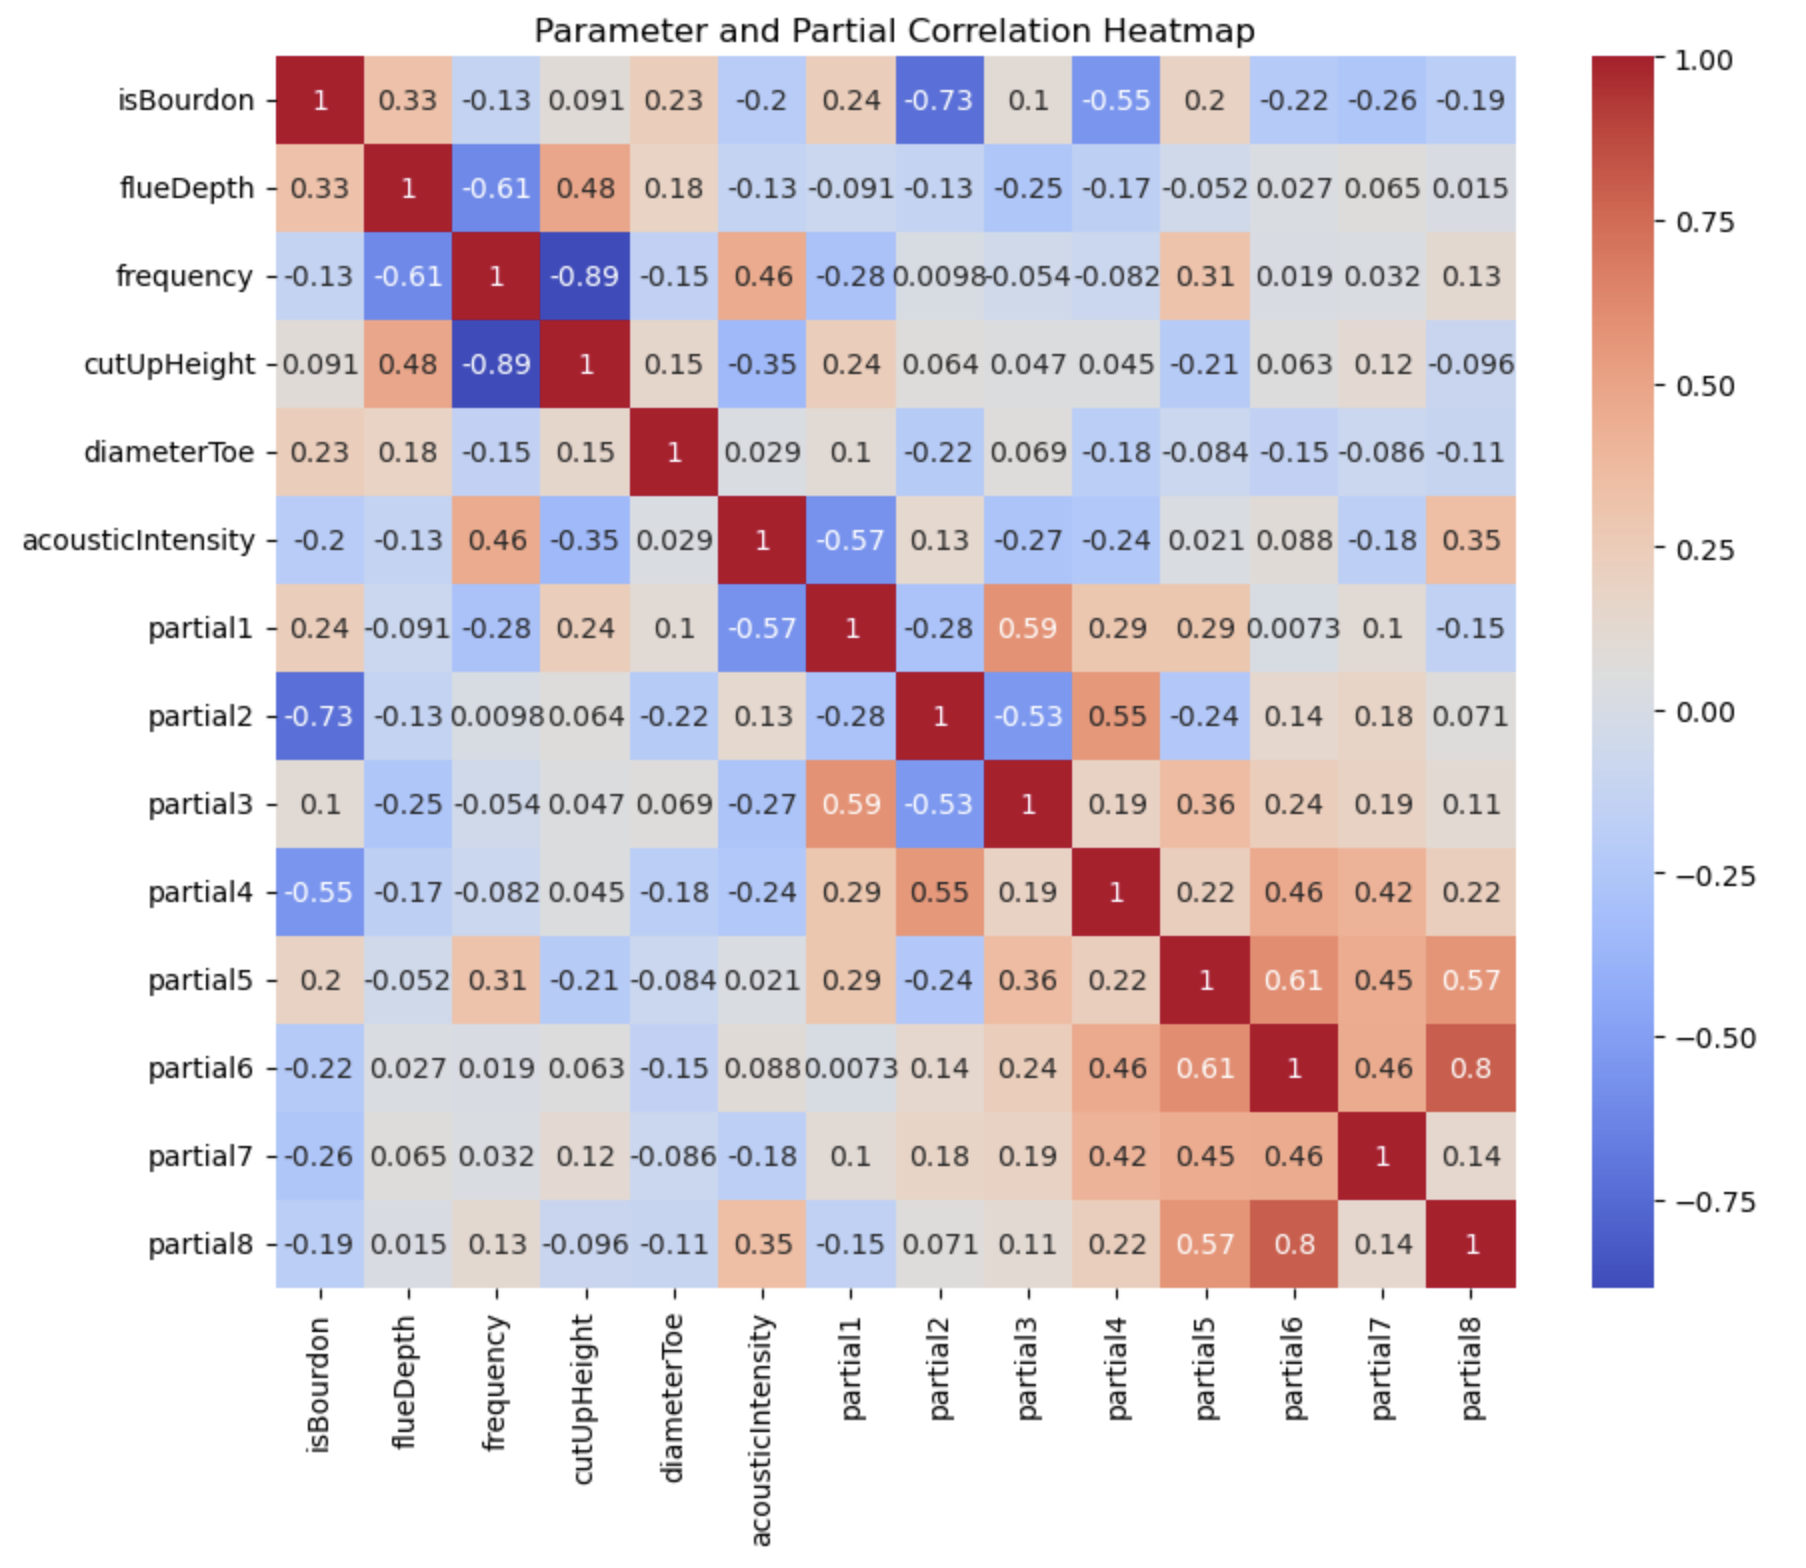
\includegraphics[width=0.8\textwidth]{pic2.png}
            \caption{Correlation matrix}
            \label{fig:distribution_partials}
        \end{figure}
    \end{frame}

    \begin{frame}
        \frametitle{Basic corrections}
        \begin{columns}
            \begin{column}{0.5\textwidth}
                \begin{alertblock}{Correlation matrix}
                    \begin{itemize}
                        \item Natural correlation between fundamental frequency
                            and dimensioning of the pipe.
                        \item Lack of observations hinders the analysis.
                    \end{itemize}
                \end{alertblock}
            \end{column}
            \begin{column}{0.5\textwidth}
                \begin{block}{Direct-naive correction}
                    Include linear term in the Ising number:
                    \[
                        \hat{\mathsf{I}} =
                        \mathsf{I}\left(1 + \frac{\mathsf{S}}{2}\right).
                    \]

                    \emph{Use Bernoulli's Law to justify the correction from
                    the physics.}
                \end{block}
            \end{column}
        \end{columns}
    \end{frame}

    \begin{frame}
        \frametitle{Deep neural network approach}
        \begin{alertblock}{Deep neural network?}
             \begin{itemize}
                 \item Few data points \(\to\) tall v/s wide DNN.
                 \item Loss function \(\to\) mean squared error + Ising
                     number.
                 \item Requires \(\sigma(p, \mathsf{I}) = (\operatorname{softmax}(p), \operatorname{softplus}(I))\).
             \end{itemize}
        \end{alertblock}
        \begin{block}{Structure}
            \begin{itemize}
                \item Input layer: 8 inputs.
                \item Hidden layers: \(n_h\) hidden layers with \(n_N\) neurons.
                \item Output layer: Ising number + first 8 partial intensities,
                    as mentioned earlier.
                \item Activation function: ReLU.
            \end{itemize}
        \end{block}
    \end{frame}

    \begin{frame}
        \frametitle{Deep neural network approach}
        \begin{block}{Training}
            \begin{itemize}
                \item Train\footnote{
                    We use \texttt{JAX/Flax/Optax} for the training.}
                    the model with 80\% of the data.
                \item Validate the model with 20\% of the data.
                \item Use Adam optimizer.
                \item Use a learning rate of \(10^{-3}\).
            \end{itemize}
        \end{block}

    \end{frame}

    \begin{frame}
        \frametitle{Deep neural network approach: Loss function}
        \begin{multline*}
            \mathcal{L}(m; \theta) =
            \sum_i \left\{
            \left(
                \mathsf{DNN}(m; \theta)(x_i)(\mathsf{I}) 
                - \mathsf{I}(x_i; \theta)
            \right)^2 \right.
            \\
            +
            \left.
            \left\lVert
                \mathsf{DNN}(m; \theta)(x_i)(p) - p_i
            \right\rVert_8^2
            \right\}
        \end{multline*}
        \begin{itemize}
            \item \(\mathsf{DNN}(m; \theta)\) is the DNN model.
            \item \(x_i\in \mathbb{R}^6\) is the input data:
                \texttt{isBourdon}, \texttt{flueDepth}, \texttt{frequency},
                \texttt{cutupHeight}, \texttt{diameterToe}, \texttt{acousticIntensity}.
            \item \(p_i\) is the output data (partial intensities).
            \item \(\mathsf{I}\) is the Ising number.
            \item \(\theta\) is the set of parameters (air pressure, air density).
        \end{itemize}
        \begin{block}{Extra}
            We have a sound simulation app, with user-labeling...
        \end{block}
    \end{frame}

    \begin{frame}
        \frametitle{Generalized additive model}
        \begin{block}{Generalized additive model}
            \begin{itemize}
                \item GAM is a generalization of the linear model.
                \item It allows for non-linear relationships between the
                    predictors and the response.
                \item It is a flexible and interpretable model.
            \end{itemize}
        \end{block}

\end{document}
